\section{Hiện tượng cảm ứng điện từ}
\subsection{Tóm tắt lí thuyết}
\begin{tomtat}
	\subsubsection{Từ thông}
	\begin{center}
		\begin{tikzpicture}
			\coordinate (O) at (0,0);
			\coordinate (A) at ($(O)+(45:2)$);
			\coordinate (B) at (4,0);
			\foreach \i in {-2,-1,...,2}{
				\draw[blue, line width=1.5pt] (-3,\i)--+(0:{-\i+2.8});
				
			}
			\draw[rotate around={-45:(O)},black, line width=1.5pt, fill=green!20!white](O) ellipse (3cm and 1.25cm);
			\foreach \i in {-2,-1,...,2}{
				\draw[blue, line width=1.5pt, -stealth] (-\i,\i)--(4,\i);	
			}
			\draw[red, -stealth, line width=1.5pt] (O)--(A);
			\fill[black] (O) circle (2pt) node [left] {O};
			\tkzMarkAngle[size=0.75cm,color=purple,line width=1.5pt](B,O,A);
			\tkzLabelAngle[color=black,pos=1.0, purple](B,O,A){$\alpha$};
			\node[blue, above] at (B) {$\vec{B}$};
			\node[red, above] at (A) {$\vec{n}$};
			\node[right] at (-0.25,-1) {$S$};
		\end{tikzpicture}
	\end{center}
	\begin{dn}
		Từ thông là đại lượng đặc trưng cho số đường sức từ xuyên qua diện tích $S$ và được xác định bởi biểu thức:
		\begin{equation}
			\Phi=BS\cos\alpha
		\end{equation}
	\end{dn}
	Trong hệ SI, từ thông có đơn vị là weber $\left(\si{\weber}\right)$.
	$$\SI{1}{\weber}=\SI{1}{\tesla\cdot\meter^2}.$$
	Trong đó:
	\begin{itemize}
		\item $\Phi$: từ thông, đơn vị trong hệ SI là weber $\left(\si{\weber}\right)$;
		\item $B$: cảm ứng từ, đơn vị trong hệ SI là tesla $\left(\si{\tesla}\right)$;
		\item $S$: diện tích mặt kín ($\si{\meter^2}$);
		\item $\alpha=\left(\vec{B},\vec{n}\right)$: góc hợp bởi vector cảm ứng từ $\vec{B}$ và vector pháp tuyến $\vec{n}$ của mặt kín.
	\end{itemize}
	\begin{luuy}
		Nếu khung dây có $N$ vòng dây được đặt trong từ trường đều, thì từ thông qua khung dây được xác định bởi biểu thức:
		$$\Phi=NBS\cos\alpha.$$
	\end{luuy}
	\subsubsection{Hiện tượng cảm ứng điện từ}
	\paragraph{Khái niệm hiện tượng cảm ứng điện từ}
	\begin{dn}
		Khi từ thông qua mặt giới hạn bởi một khung dây dẫn kín biến thiên thì trong khung dây xuất hiện dòng điện cảm ứng. Hiện tượng này được gọi là hiện tượng cảm ứng điện từ.
	\end{dn}
	\paragraph{Định luật Lenz về chiều dòng điện cảm ứng}
	\begin{dl}
		Dòng điện cảm ứng qua khung dây dẫn kín có chiều sao cho từ trường do nó sinh ra (từ trường cảm ứng) có tác dụng chống lại sự biến thiên từ thông qua chính khung dây đó.
	\end{dl}
	\begin{center}
		\includegraphics[width=0.45\linewidth]{figs/VN12-Y24-PH-SYL-020-1}
		\captionof{figure}{Chiều dòng điện cảm ứng $i_c$ qua khung dây dẫn kín khi đưa nam châm (a) lại gần và (b) ra xa khung dây}
	\end{center}
	\subsubsection{Định luật Faraday về suất điện động cảm ứng}
	\begin{dl}
		Độ lớn suất điện động cảm ứng trong khung dây dẫn kín tỉ lệ với tốc độ biến thiên từ thông qua diện tích giới hạn bởi khung dây.\\
		Trong hệ SI, độ lớn suất điện động cảm ứng được xác định bằng biểu thức:
		\begin{equation}
			\left|e_c\right|=\left|\dfrac{\Delta \Phi}{\Delta t}\right|
		\end{equation}
	\end{dl}
	Trong đó:
	\begin{itemize}
		\item $\left|e_c\right|$: độ lớn suất điện động cảm ứng, đơn vị trong hệ SI là volt $\left(\si{\volt}\right)$;
		\item $\Delta\Phi$: độ biến thiên từ thông, đơn vị trong hệ SI là weber $\left(\si{\weber}\right)$;
		\item $\Delta t$: khoảng thời gian từ thông biến thiên, đơn vị trong hệ SI là giây $\left(\si{\second}\right)$.
	\end{itemize}
	\begin{luuy}
		Khi kết hợp với nội dung định luật Lenz, biểu thức định luật Faraday được viết lại:
		\begin{equation}
			e_c=-\dfrac{\Delta \Phi}{\Delta t}
		\end{equation}
		Trong trường hợp khung dây có $N$ vòng dây thì:
		\begin{equation}
			e_c=-N\dfrac{\Delta \Phi}{\Delta t}
		\end{equation}
	\end{luuy}
	\subsubsection{Một số ứng dụng của hiện tượng cảm ứng điện từ}
	\paragraph{Guitar điện}
	\begin{minipage}{0.5\textwidth}
		Bộ cảm ứng (pickup) của guitar điện gồm một cuộn dây và một nam châm vĩnh cửu, được đặt gần dây đàn guitar bằng kim loại có thể nhiễm từ. Khi gảy đàn, đoạn dây gần nam châm bị nhiễm từ, dao động và tạo ra sự biến thiên từ thông qua cuộn dây của bộ cảm ứng, từ đó tạo ra suất điện động cảm ứng. Tín hiệu điện được đưa đến một bộ khuếch đại và loa, tạo ra sóng âm thanh mà chúng ta nghe được.
	\end{minipage}
	\hfill
	\begin{minipage}{0.5\textwidth}
		\centering
		\includegraphics[width=0.55\linewidth]{figs/VN12-Y24-PH-SYL-021-1}
	\end{minipage}
	\paragraph{Dynamo xe đạp}
	Khi bánh xe quay, núm dẫn  động và nam châm cũng quay theo, do đó từ thông qua cuộn dây biến thiên. Lúc này, trong cuộn dây xuất hiện dòng điện cảm ứng và thắp sáng bóng đèn.
	\begin{center}
		\includegraphics[width=0.6\linewidth]{figs/VN12-Y24-PH-SYL-021-2}
		\captionof{figure}{a) Dynamo trên xe đạp; b) Cấu tạo của dynamo trên xe đạp.}
	\end{center}
	\subsubsection{Mô hình sóng điện từ}
	\paragraph{Điện từ trường}
	\begin{dn}
		Trong vùng không gian có từ trường biến thiên theo thời gian thì trong vùng đó xuất hiện một điện trường xoáy; ngược lại, trong vùng không gian có điện trường biến thiên theo thời gian thì trong vùng đó xuất hiện một từ trường biến thiên theo thời gian. Do đó, điện trường biến thiên và từ trường biến thiên theo thời gian chuyển hoá lẫn nhau và cùng tồn tại trong không gian, được gọi là điện từ trường.
	\end{dn}
	\begin{center}
		\includegraphics[width=0.6\linewidth]{figs/VN12-Y24-PH-SYL-021-3}
		\captionof{figure}{a) Điện trường biến thiên gây ra từ trường biến thiên; b) Từ trường biến thiên gây ra điện trường biến thiên.}
	\end{center}
	\paragraph{Mô hình sóng điện từ}
	\begin{center}
		\includegraphics[width=0.8\linewidth]{figs/VN12-Y24-PH-SYL-021-4}
		\captionof{figure}{a) Mô hình sự lan truyền sóng điện từ; b) Minh hoạ quy tắc vặn đinh ốc.}
	\end{center}
	Trong quá trình lan truyền sóng điện từ, tại một điểm có
	\begin{itemize}
		\item vector cường độ điện trường $\vec{E}$ và vector cảm ứng từ $\vec{B}$ luôn vuông góc với nhau và vuông góc với phương truyền sóng $\Rightarrow $ sóng điện từ là sóng ngang;
		\item điện trường và từ trường biến thiên cùng pha.
	\end{itemize}
\begin{noidung}{Quy tắc vặn đinh ốc để xác định chiều truyền sóng điện từ}
	Quay đinh ốc theo chiều từ vector cường độ điện trường đến vector cảm ứng từ thì chiều tiến của đinh ốc là chiều lan truyền của sóng điện từ.
\end{noidung}
\end{tomtat}

\subsection{Ví dụ minh hoạ}
\begin{dang}{Xác định từ thông gửi qua khung dây}
	\end{dang}
\begin{vd}
		Một vòng dây phẳng giới hạn diện tích $S=\SI{5}{\centi\meter^2}$ đặt trong từ trường đều có cảm ứng từ $B=\SI{0.1}{\tesla}$. Mặt phẳng vòng dây làm thành với $\vec{B}$ một góc $\alpha=\SI{30}{\degree}$. Tính từ thông qua $S$.
		\loigiai{Góc hợp bởi $\vec{B}$ và vector pháp tuyến $\vec{n}$ của mặt phẳng khung dây $\left(\vec{B},\vec{n}\right)=\SI{90}{\degree}-\alpha=\SI{60}{\degree}.$\\
			Từ thông qua tiết diện $S$:
			$$\Phi=BS\cos\left(\vec{B}, \vec{n}\right)=\left(\SI{0.1}{\tesla}\right)\cdot\left(\SI{5E-4}{\meter^2}\right)\cos\SI{60}{\degree}=\SI{2.5E-5}{\weber}.$$}
\end{vd}
% ==================================
\begin{vd}
		Một khung dây phẳng giới hạn diện tích $S=\SI{5}{\centi\meter^2}$ gồm 20 vòng dây đặt trong từ trường đều  có cảm ứng từ $B=\SI{0.1}{\tesla}$ sao cho mặt phẳng khung dây hợp với vector cảm ứng từ một góc $\SI{60}{\degree}$. Tính từ thông qua diện tích giới hạn bởi khung dây.
		\loigiai{Góc hợp bởi vector cảm ứng từ $\vec{B}$ và vector pháp tuyến $\vec{n}$ là $\left(\vec{B},\vec{n}\right)=\SI{90}{\degree}-\SI{60}{\degree}=\SI{30}{\degree}.$\\
			Từ thông qua diện tích giới hạn bởi khung dây:
			$$\Phi=NBS\cos\left(\vec{B},\vec{n}\right)=\SI{8.66E-4}{\weber}.$$}
\end{vd}

\begin{dang}{Vận dụng định luật Lenz xác định chiều dòng điện cảm ứng}
	\end{dang}
% ====================
\begin{vd}
		Đặt một thanh nam châm thẳng ở gần một khung dây kín ABCD như hình vẽ.
		\begin{center}
			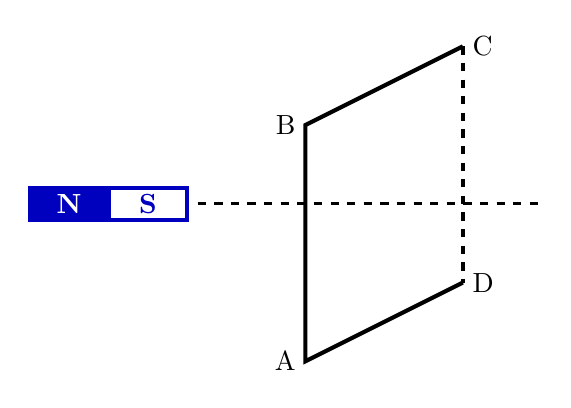
\begin{tikzpicture}
				\coordinate (B) at (0,0);
				\coordinate (A) at (0,-3);
				\coordinate (C) at (2,1);
				\coordinate (D) at (2,-2);
				\coordinate (N) at (-3cm,-1cm);
				\coordinate (S) at (-2cm,-1cm);
				\draw[dashed, line width=1pt] (S)--(3,-1);
				\node[draw,color= blue!75!black, line width=1.5pt, fill=blue!75!black, rectangle, minimum width=1cm, minimum height=0.4cm, anchor=center] at(N) {};
				\node[draw,color= blue!75!black, line width=1.5pt, fill=white, rectangle, minimum width=1cm, minimum height=0.4cm, anchor=center] at(S) {};
				\draw[line width=1.5pt] (C)--(B)--(A)--(D);
				\draw[line width=1.5pt, dashed] (C)--(D);
				\node[left] at (A) {A};
				\node[left] at (B) {B};
				\node[right] at (C) {C};
				\node[right] at (D) {D};
				\node[color=white] at (N) {\bfseries N};
				\node[color=blue!75!black] at (S) {\bfseries S};
			\end{tikzpicture}
		\end{center}
		Xác định chiều của dòng điện cảm ứng xuất hiện trong khung dây trong các trường hợp sau:
		\begin{enumerate}[label=\alph*)]
			\item Đưa nam châm lại gần khung dây.
			\item Kéo nam châm ra xa khung dây.
		\end{enumerate}
		\loigiai{\begin{enumerate}[label=\alph*)]
				\item Đưa nam châm lại gần khung dây, từ thông qua khung dây tăng nên $\vec{B}_c\uparrow\downarrow \vec{B}_0$.
				\begin{center}
					\begin{tikzpicture}
						\coordinate (B) at (0,0);
						\coordinate (A) at (0,-3);
						\coordinate (C) at (2,1);
						\coordinate (D) at (2,-2);
						\coordinate (N) at (-3cm,-1cm);
						\coordinate (S) at (-2cm,-1cm);
						\draw[dashed, line width=1pt] (S)--(3,-1);
						\draw[-stealth, blue, line width=1.5pt] (N)--+(-2,0);
						\draw[-stealth, line width=1.5pt] (S)--+(1.5,0);
						\draw[-stealth, red, line width=1.5pt] (1,-1)--+(1.5,0);
						\node[draw,color= blue!75!black, line width=1.5pt, fill=blue!75!black, rectangle, minimum width=1cm, minimum height=0.4cm, anchor=center] at(N) {};
						\node[draw,color= blue!75!black, line width=1.5pt, fill=white, rectangle, minimum width=1cm, minimum height=0.4cm, anchor=center] at(S) {};
						\draw[line width=1.5pt,decoration={markings, mark=at position 0.5 with {\arrow{stealth}}},
						postaction={decorate}
						] (C)--(B)--(A)--(D);
						\draw[line width=1.5pt, dashed] (C)--(D);
						\node[above,blue] at ($(N)+(-2,0)$) {$\vec{B}_0$};
						\node[above] at ($(S)+(1.5,0)$) {$\vec{v}_0$};
						\node[above, red] at (2.5,-1) {$\vec{B}_c$};
						\node[right] at ($(A)!0.5!(B)$) {$i_c$};
						\node[left] at (A) {A};
						\node[left] at (B) {B};
						\node[right] at (C) {C};
						\node[right] at (D) {D};
						\node[color=white] at (N) {\bfseries N};
						\node[color=blue!75!black] at (S) {\bfseries S};
					\end{tikzpicture}
				\end{center}
				\item Đưa nam châm ra xa khung dây, từ thông qua khung dây giảm nên $\vec{B}_c\uparrow\uparrow \vec{B}_0$.
				\begin{center}
					\begin{tikzpicture}
						\coordinate (B) at (0,0);
						\coordinate (A) at (0,-3);
						\coordinate (C) at (2,1);
						\coordinate (D) at (2,-2);
						\coordinate (N) at (-3cm,-1cm);
						\coordinate (S) at (-2cm,-1cm);
						\draw[dashed, line width=1pt] (S)--(3,-1);
						\draw[-stealth, blue, line width=1.5pt] (N)--+(-2,0);
						\draw[-stealth, line width=1.5pt] (N)--+(-1,0);
						\draw[-stealth, red, line width=1.5pt] (1,-1)--+(-1.5,0);
						\node[draw,color= blue!75!black, line width=1.5pt, fill=blue!75!black, rectangle, minimum width=1cm, minimum height=0.4cm, anchor=center] at(N) {};
						\node[draw,color= blue!75!black, line width=1.5pt, fill=white, rectangle, minimum width=1cm, minimum height=0.4cm, anchor=center] at(S) {};
						\draw[line width=1.5pt,decoration={markings, mark=at position 0.5 with {\arrow{stealth}}},
						postaction={decorate}
						] (D)--(A)--(B)--(C);
						\draw[line width=1.5pt, dashed] (C)--(D);
						\node[above,blue] at ($(N)+(-2,0)$) {$\vec{B}_0$};
						\node[above] at ($(N)+(-1,0)$) {$\vec{v}_0$};
						\node[above, red] at (-0.5,-1) {$\vec{B}_c$};
						\node[right] at ($(A)!0.5!(B)$) {$i_c$};
						\node[left] at (A) {A};
						\node[left] at (B) {B};
						\node[right] at (C) {C};
						\node[right] at (D) {D};
						\node[color=white] at (N) {\bfseries N};
						\node[color=blue!75!black] at (S) {\bfseries S};
					\end{tikzpicture}
				\end{center}
		\end{enumerate}	}
\end{vd}
% ================================
\begin{vd}
		Xác định chiều dòng điện cảm ứng xuất hiện trong mạch ABCD khi dịch chuyển mạch ABCD ra xa dòng điện $I$ thẳng, dài vô hạn. Biết mạch ABCD và dòng điện $I$ luôn nằm trong cùng mặt phẳng.
		\begin{center}
			\begin{tikzpicture}
				\coordinate(O) at(0,0);
				\node[draw, rectangle, line width=1.5pt, minimum height=3cm, minimum width=2cm] at (O) {};
				\draw[line width=1.5pt, blue, decoration={markings, mark=at position 0.5 with {\arrow{stealth}}},
				postaction={decorate}
				] (-2,-3)--(-2,3);
				\draw[line width=1.5pt, -stealth] (1,0)--+(1,0);
				\node[left,blue] at(-2,0) {$I$};
				\node[above] at (2,0) {$\vec{v}_0$};
				\node[above] at (-1,1.5) {A};
				\node[above] at (1,1.5) {B};
				\node[below] at (1,-1.5) {C};
				\node[below] at (-1,-1.5) {D};
			\end{tikzpicture}
		\end{center}
		\loigiai{\begin{center}
				\begin{tabular}{M{5cm}L{11cm}}
					\begin{tikzpicture}
						\coordinate(O) at(0,0);
						\node[draw, rectangle, line width=1.5pt, minimum height=3cm, minimum width=2cm, decoration={markings, mark=at position 0.1 with {\arrowreversed{stealth}}},
						decoration={markings, mark=at position 0.6 with {\arrowreversed{stealth}}},
						postaction={decorate}] at (O) {};
						\draw[line width=1.5pt, blue, decoration={markings, mark=at position 0.5 with {\arrow{stealth}}},
						postaction={decorate}
						] (-2,-2)--(-2,2);
						\draw[line width=1.5pt, -stealth] (1,0)--+(1,0);
						\node[blue] at (0,-0.5) {\LARGE$\otimes$};
						\node[red] at (0,0.5) {\LARGE$\otimes$};
						\node[blue, right] at (0.25,-0.5) {$\vec{B}_0$};
						\node[red, right] at (0.25,0.5) {$\vec{B}_c$};
						\node[left,blue] at(-2,0) {$I$};
						\node[above] at (2,0) {$\vec{v}_0$};
						\node[above] at (-1,1.5) {A};
						\node[above] at (1,1.5) {B};
						\node[below] at (1,-1.5) {C};
						\node[below] at (-1,-1.5) {D};
						\node[above] at (0,1.5) {$i_c$};
					\end{tikzpicture} & Dòng điện thẳng $I$ gây ra trong mạch ABCD từ trường  có các đường cảm ứng từ $\vec{B}_0$  hướng vào mặt phẳng ABCD.\newline
					Khi di chuyển khung ra xa dây, từ thông qua mạch giảm nên $\vec{B}_c$ do $i_c$ tạo ra cùng chiều $\vec{B}_0$. Do đó, mặt ABCD là mặt Nam nên $i_c$ cùng chiều kim đồng hồ theo chiều ABCD.\\
				\end{tabular}
			\end{center}
		}
\end{vd}
\begin{dang}{Giải thích được một số ứng dụng của hiện tượng cảm ứng điện từ}
\end{dang}
\begin{vd}
		Cho một đĩa kim loại dao động trong không khí, đĩa sẽ dao động trong một thời gian xác định. Khi cho đĩa dao động giữa hai cực từ của một nam châm thì thời gian đĩa dao động sẽ ngắn hơn. Hiện tượng này được ứng dùng để hãm chuyển động, đặc biệt là chuyển động quay của một bộ phận nào đó trong một số thiết bị. Em hãy giải thích cơ chế của hiện tượng trên.
		\begin{center}
			\includegraphics[width=0.15\linewidth]{figs/VN12-Y24-PH-SYL-021-5}
		\end{center}
		\loigiai{Khi đĩa đi vào từ trường, nó cắt các đường sức từ và do đó trong đĩa xuất hiện suất điện động cảm ứng. Vì đĩa là chất dẫn điện nên suất điện động cảm ứng tạo ra dòng điện trong đĩa. Những dòng điện này được gọi là dòng điện xoáy (dòng điện Foucault). Chúng có đặc điểm là chạy theo các đường cong kín trong khối vật dẫn.\\
			Theo định luật Lenz, các dòng điện cảm ứng chạy trong đĩa sẽ tạo ra lực cản trở chuyển động, làm cho dao động bị tắt dần nhanh.}
\end{vd}
% =====================================
\begin{vd}
		Hình bên là một đèn pin có thể được sạc lại bằng cách lắc đèn pin theo trục dọc của nó.
		\begin{center}
			\includegraphics[width=0.4\linewidth]{figs/VN12-Y24-PH-SYL-021-6}
		\end{center}
		\begin{enumerate}[label=\alph*)]
			\item Tại sao khi lắc đèn thì pin được sạc (nạp điện)?
			\item Nêu cách để thời gian sạc nhanh hơn.
		\end{enumerate}
		\loigiai{\begin{enumerate}[label=\alph*)]
				\item Khi lắc đèn pin, nam châm sẽ dao động qua lại trong cuộn dây, làm từ trường qua cuộn dây tăng giảm dẫn đến từ thông qua cuộn dây biến đổi và làm xuất hiện suất điện động cảm ứng trong cuộn dây. Suất điện động này gây ra hiệu điện thế ở hai đầu cuộn dây. Hiệu điện thế này tạo ra dòng điện để sạc điện cho pin.
				\item Để thời gian sạc nhanh hơn cần tăng hiệu điện thế, bằng cách:
				\begin{itemize}
					\item Cách 1: Cho nam châm chuyển động nhanh hơn (lắc nhanh);
					\item Cách 2: Tăng số vòng dây trên cuộn dây hoặc từ trường của nam châm mạnh hơn. Cách này phụ thuộc vào nhà sản xuất đèn pin.
				\end{itemize}
		\end{enumerate}	}
\end{vd}
\begin{dang}{Vận dụng định luật Faraday tính được suất điện động cảm ứng}
\end{dang}
\begin{vd}
	Một đĩa kim loại được chế tạo để quay với tốc độ 20 vòng/giây quanh một trục đi qua tâm và vuông góc với mặt phẳng của nó. Đĩa được đặt trong từ trường đều có độ lớn cảm ứng từ là $\SI{0.2}{\tesla}$ và song song với trục quay.
	\begin{enumerate}[label=\alph*)]
		\item Đĩa có bán kính $\SI{30}{\centi\meter}$, tính diện tích quét được trong một giây bởi bán kính của đĩa.
		\item Tính từ thông gửi qua đĩa trong một giây.
		\item Tính suất điện động cảm ứng xuất hiện khi đĩa quay.
	\end{enumerate}
	\loigiai{\begin{enumerate}[label=\alph*)]
			\item Diện tích quét được trong một giây bởi bán kính của đĩa:
			$$S=N\cdot\pi R^2=nt\pi R^2=\left(\SI{20}{\text{vòng}/\second}\right)\cdot\left(\SI{1}{\second}\right)\cdot\pi\cdot\left(\SI{0.3}{\meter}\right)^2\approx\SI{5.65}{\meter^2}.$$
			\item Từ trường đều, song song với trục quay nên $\alpha=\left(\vec{n},\vec{B}\right)=\SI{0}{\degree}$.\\
			Từ thông gửi qua tiết diện đĩa trong 1 giây:
			$$\Phi=BS\cos\alpha=\left(\SI{0.2}{\tesla}\right)\cdot\left(\SI{5.65}{\meter^2}\right)\cdot\cos\SI{0}{\degree}=\SI{1.13}{\weber}.$$
			\item Suất điện động cảm ứng xuất hiện trong đĩa:
			$$e_c=-\dfrac{\Delta \Phi}{\Delta t}=-\dfrac{\Phi-\Phi_0}{\Delta t}=-\dfrac{\SI{1.13}{\weber}-0}{\SI{1}{\second}}=-\SI{1.13}{\volt}.$$
	\end{enumerate}}
\end{vd}
% ============================================================
\begin{vd}
	Một cuộn dây có 50 vòng và tiết diện $\SI{8.0E-4}{\meter^2}$. Cuộn dây được đặt vuông góc với từ trường đều có độ lớn cảm ứng từ là $\SI{0.2}{\tesla}$.
	\begin{enumerate}[label=\alph*)]
		\item Tính suất điện động cảm ứng trung bình trong cuộn dây, khi từ trường giảm về 0 trong $\SI{50}{\milli\second}$.
		\item Tính suất điện động cảm ứng trung bình trong cuộn dây, khi từ trường đảo chiều trong $\SI{50}{\milli\second}$.
	\end{enumerate}	
		\loigiai{\begin{enumerate}[label=\alph*)]
				\item Suất điện động cảm ứng xuất hiện trong cuộn dây khi từ trường giảm về 0 trong $\SI{50}{\milli\second}$:
				$$e_c=-N\dfrac{\Delta \Phi}{\Delta t}=-NS\dfrac{\Delta B}{\Delta t}\cos\alpha=-50\cdot\left(\SI{8.0E-4}{\meter^2}\right)\dfrac{\left(0-\SI{0.2}{\tesla}\right)}{\SI{50E-3}{\second}}\cdot\cos\SI{0}{\degree}=\SI{0.16}{\volt}.$$
				\item Suất điện động cảm ứng xuất hiện trong cuộn dây nếu từ trường đảo chiều trong $\SI{50}{\milli\second}$:
				$$e_c=-N\dfrac{\Delta \Phi}{\Delta t}=-NBS\dfrac{\left(\cos\SI{180}{\degree}-\cos\SI{0}{\degree}\right)}{\Delta t}=-50\cdot\left(\SI{0.2}{\tesla}\right)\cdot\left(\SI{8.0E-4}{\meter^2}\right)\cdot\dfrac{\left(\cos\SI{180}{\degree}-\cos\SI{0}{\degree}\right)}{\SI{50E-3}{\second}}=\SI{0.32}{\volt}.$$
		\end{enumerate}	}
\end{vd}
% =================================
\begin{vd}
		Đồ thị sau đây biểu diễn sự biến thiên của từ thông toàn phần theo thời gian trong một cuộn dây phẳng:
		\begin{center}
			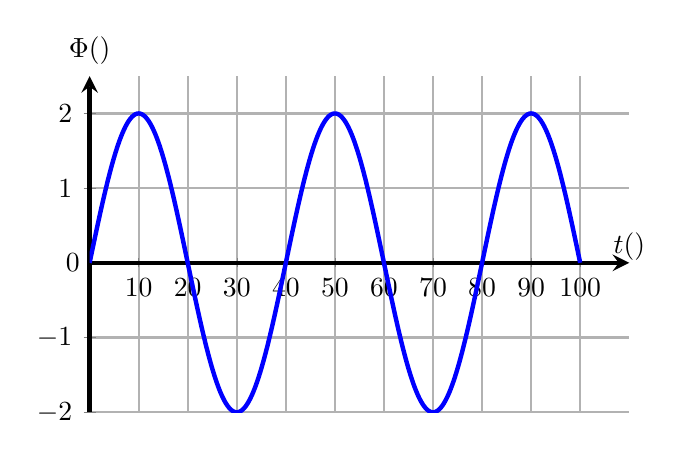
\begin{tikzpicture}  
				\begin{axis}[  ultra thick, yscale=0.75,
					xmin=0,  
					xmax=110,  
					xtick={0,10,...,100},
					ytick={-2,-1,...,2},
					minor x tick num=0,
					minor y tick num=0,
					ymin=-2,  
					ymax=2.5, 
					samples=300,
					axis lines=center, 
					grid style={step=1, line width =0.4pt, color=gray!30!white},
					grid=both,
					major grid style={line width=0.8pt,gray!60!white},
					xlabel=$\xsi{t}{\left(\si{\milli\second}\right)}$, 		ylabel=$\xsi{\Phi}{\left(\si{\weber}\right)}$,
					every axis y label/.style={at=(current axis.above origin),anchor=south},  
					every axis x label/.style={at=(current axis.right of origin),anchor=west, below=0.1cm},  ]
					\addplot [ultra thick, blue, smooth, domain=0:100] {2*cos(deg(pi*x/20-pi/2))} ;  
				\end{axis}   \node[left] at (0,1.9) {0};
			\end{tikzpicture}
			
		\end{center}
		\begin{enumerate}[label=\alph*)]
			\item Hãy cho biết các thời điểm suất điện động cảm ứng trong cuộn dây có độ lớn cực đại, có giá trị bằng 0.
			\item Biết từ thông qua cuộn dây biến đổi chỉ do từ trường qua cuộn dây thay đổi và từ trường này có đường cảm ứng từ vuông góc mặt phẳng cuộn dây. Nếu diện tích mặt cắt ngang của cuộn dây là $\SI{1.6E-2}{\meter^2}$ và cuộn dây có 500 vòng dây, hãy tính giá trị lớn nhất của cường độ từ trường.
		\end{enumerate}
		\loigiai{\begin{enumerate}[label=\alph*)]
				\item Từ $\left|e\right|=\left|-N\cdot\dfrac{\Delta \Phi}{\Delta t}\right|$, ta thấy suất điện động cảm ứng trong cuộn dây có độ lớn cực đại khi tốc độ biến thiên của từ thông qua cuộn dây đạt giá trị cực đại.\\
				Dựa vào đồ thị, tốc độ biến thiên của từ thông đạt cực đại tại các thời điểm đồ thị có độ dốc lớn nhất.
				\begin{itemize}
					\item Tại các thời điểm $\SI{0}{\milli\second}$, $\SI{20}{\milli\second}$, $\SI{40}{\milli\second}$, $\SI{80}{\milli\second}$ hoặc $\SI{100}{\milli\second}$ thì suất điện động có giá trị cực đại, lúc này từ thông bằng 0.
					\item  Tại các thời điểm $\SI{10}{\milli\second}$, $\SI{30}{\milli\second}$, $\SI{50}{\milli\second}$, $\SI{70}{\milli\second}$ hoặc $\SI{90}{\milli\second}$ thì suất điện động trong cuộn dây bằng 0, lúc này từ thông có độ lớn cực đại.
				\end{itemize}
				\item Từ $\Phi=NBS\Rightarrow B_\text{max}=\dfrac{\Phi_\text{max}}{NS}=\dfrac{\left(\SI{2}{\weber}\right)}{500\cdot\left(\SI{1.6E-2}{\meter^2}\right)}=\SI{0.25}{\tesla}.$
		\end{enumerate}	}
\end{vd}
\subsection{Bài tập}
\subsubsection{Trắc nghiệm nhiều phương án lựa chọn}
\setcounter{ex}{0}
\Opensolutionfile{ans}[ans/VN12-Y24-PH-SYL-020P-TN]
% ===================================================================
\begin{ex}
	Trong các phát biểu sau, phát biểu nào là \textbf{đúng}?
	\begin{enumerate}[label=(\arabic*)]
		\item Độ lớn từ thông qua một mạch kín càng lớn khi số lượng đường sức từ xuyên qua mạch kín này càng nhỏ.
		\item Đơn vị của từ thông là tesla $\left(\si{\tesla}\right)$.
		\item Khi từ thông qua mặt giới hạn bởi một khung dây dẫn kín biến thiên theo thời gian thì trong khung dây xuất hiện dòng điện cảm ứng.
		\item Trong hiện tượng cảm ứng điện từ, dòng điện cảm ứng sinh ra trong một khung dây dẫn kín có tác dụng chống lại sự biến thiên từ thông qua chính khung dây đó.
	\end{enumerate}
	\choice
	{(1), (2)}
	{(2), (3)}
	{\True (3), (4)}
	{(1),(4)}
	\loigiai{
		
	}
\end{ex}

% ===================================================================
\begin{ex}
	Phát biểu nào sau đây về từ thông là \textbf{không đúng}?
	\choice
	{\True Từ thông là đại lượng vector, được xác định bằng số đường sức từ xuyên qua tiết diện của cuộn dây}
	{Từ thông là đại lượng vô hướng, được sử dụng để diễn tả số đường sức từ xuyên qua diện tích $S$ nào đó}
	{Đơn vị của từ thông là weber, kí hiệu là $\si{\weber}$}
	{Từ thông qua diện tích $S$ nào đó bằng không khi vector pháp tuyến của diện tích $S$ vuông góc với vector cảm ứng từ của từ trường}
	\loigiai{	
	}
\end{ex}
% ===================================================================
\begin{ex}
	Phát biểu nào sau đây là \textbf{đúng} khi nói về hiện tượng cảm ứng điện từ?
	\choice
	{\True Hiện tượng cảm ứng điện từ chỉ tồn tại trong khoảng thời gian có từ thông qua mạch kín biến thiên}
	{Khi có từ thông biến thiên qua cuộn dây dẫn thì luôn có dòng điện cảm ứng xuất hiện trong cuộn dây, ngay cả khi cuộn dây không kín}
	{Hiện tượng cảm ứng điện từ không xảy ra trong khối vật dẫn, kể cả khi có từ thông biến thiên qua khối vật dẫn đó}
	{Dòng điện cảm ứng chạy trong cuộn dây dẫn kín không gây ra tác dụng nhiệt đối với cuộn dây}
	\loigiai{}
\end{ex}
% ===================================================================
\begin{ex}
	Cách nào sau đây \textbf{không làm} cho từ thông qua tiết diện vòng dây dẫn kín biến thiên?
	\choice
	{Quay vòng dây cắt ngang các đường cảm ứng từ của nam châm vĩnh cửu}
	{\True Dịch chuyển nam châm sao cho các đường sức từ dịch chuyển song song với mẳt phẳng khung dây}
	{Đặt mặt phẳng cuộn dây cạnh nam châm điện xoay chiều}
	{Cho nam châm vĩnh cửu rơi qua lòng cuộn dây}
	\loigiai{}
\end{ex}
% ===================================================================
\begin{ex}
	Một vòng dây dẫn được đặt nằm theo phương ngang trong từ trường có cảm ứng từ $\vec{B}$, trong vòng dây dẫn xuất hiện dòng điện cảm ứng theo chiều kim đồng hồ (nhìn từ trên xuống mặt phẳng vòng dây). Phát biểu nào sau đây về độ lớn và chiều của cảm ứng từ là \textbf{đúng}?
	\choice
	{Có độ lớn không đổi, hướng thẳng đứng xuống dưới}
	{Có độ lớn không đổi, hướng thẳng đứng lên trên}
	{Có độ lớn tăng dần, hướng thẳng đứng xuống dưới}
	{\True Có độ lớn giảm dần, hướng thẳng đứng xuống dưới}
	\loigiai{}
\end{ex}


% ===================================================================
\begin{ex}
	Một học sinh đo cường độ dòng điện chạy trong ống dây khi di chuyển cực bắc của thanh nam châm lại gần ống dây. Cường độ dòng điện sẽ tăng khi
	\choice
	{\True sử dụng thanh nam châm mạnh hơn}
	{di chuyển nam châm theo hướng ngược lại}
	{di chuyển cuộn dây, giữ yên nam châm}
	{di chuyển cực nam của thanh nam châm}
	\loigiai{}
\end{ex}

% ===================================================================
\begin{ex}
	Cách nào sau đây \textbf{không} tạo ra suất điện động cảm ứng?
	\choice
	{Di chuyển một dây dẫn giữa các cực của nam châm}
	{Di chuyển một thanh nam châm ra khỏi một ống dây dẫn}
	{\True Giữ cố định một dây dẫn giữa hai cực của nam châm}
	{Làm quay một khung dây dẫn trong từ trường}
	\loigiai{}
\end{ex}
% ===================================================================
\begin{ex}
	Ở thí nghiệm về hiện tượng cảm ứng điện từ theo thiết kế thí nghiệm hình bên. Khi tăng tốc độ di chuyển thanh nam châm, dòng điện trong ống dây
	\begin{center}
		\includegraphics[width=0.4\linewidth]{figs/VN12-Y24-PH-SYL-020P-17}
	\end{center}
	\choice
	{\True có độ lớn tăng lên}
	{có độ lớn giảm đi}
	{có độ lớn không đổi}
	{đảo ngược chiều}
	\loigiai{}
\end{ex}
% ===================================================================
\begin{ex}
	Ví dụ nào sau đây \textbf{không phải} là ví dụ về cảm ứng điện từ?
	\choice
	{Một khung dây quay trong từ trường sẽ tạo ra suất điện động trong khung dây dẫn đó}
	{Một nam châm di chuyển lại gần và ra xa ống dây dẫn sẽ tạo ra một điện áp trong ống dây dẫn đó}
	{\True Một dây dẫn có dòng điện chịu một lực khi được đặt giữa hai cực của một nam châm}
	{Một sự chênh lệch điện thế được tạo ra trên một dây dẫn chuyển động trong từ trường}
	\loigiai{}
\end{ex}
% ===================================================================
\begin{ex}
	Phát biểu nào sau đây nói đến hiện tượng cảm ứng điện từ?
	\choice
	{Sự tạo ra suất điện động qua một dây dẫn khi không có chuyển động giữa dây dẫn và từ trường}
	{Sự tạo ra suất điện động qua một dây dẫn khi có sự chuyển động tương đối giữa dây dẫn và dòng điện cảm ứng}
	{Sự tạo ra suất điện động qua một dây dẫn khi không có chuyển động giữa dây dẫn và dòng điện cảm ứng}
	{\True Sự tạo ra suất điện động qua một dây dẫn khi có chuyển động tương đối giữa dây dẫn và từ trường}
	\loigiai{}
\end{ex}
% ===================================================================
\begin{ex}
	Trong hiện tượng cảm ứng điện từ, suất điện động cảm ứng sinh ra do sự biến thiên của từ thông theo thời gian được xác định bằng biểu thức
	\choice
	{\True $e=-N \frac{\Delta \Phi}{\Delta t}$}
	{$e=N \frac{\Delta \Phi}{\Delta t}$}
	{$e=-N \Delta \Phi \Delta t$}
	{$e=N \Delta \Phi \Delta t$}
	\loigiai{
		
	}
\end{ex}
% ===================================================================
\begin{ex}
	Xét một vòng kim loại đang chuyển động đều từ A đến E như hình \ref{fig:20P-1}. Trong quá trình chuyển động, vòng đi vào vùng từ trường đều abcd có các đường sức từ vuông góc với mặt phẳng vòng dây. Trong quá trình chuyển động, số lượng đường sức từ xuyên qua vòng kim loại này giảm dần trong giai đoạn nào?
	\begin{center}
		\includegraphics[width=0.4\linewidth]{figs/VN12-Y24-PH-SYL-020P-1}
		\captionof{figure}{}
		\label{fig:20P-1}
	\end{center}
	\choice
	{Từ A đến B}
	{Từ B đến C}
	{Từ C đến D}
	{\True Từ D đến E}
	\loigiai{
		
	}
\end{ex}
% ===================================================================
\begin{ex}
	Khi nam châm dịch chuyển ra xa ống dây, trong ống dây có dòng điện cảm ứng. Nếu nhìn từ phía thanh nam châm vào đầu ống dây, phát biểu nào sau đây là \textbf{đúng}?
	\begin{center}
		\includegraphics[width=0.4\linewidth]{figs/VN12-Y24-PH-SYL-020P-18}
	\end{center}
	\choice
	{Dòng điện chạy theo chiều kim đồng hồ, đầu 1 là cực bắc của ống dây và hút cực bắc của thanh nam châm}
	{Dòng điện chạy ngược chiều kim đồng hồ, đầu 1 là cực bắc của ống dây và đẩy cực nam của thanh nam châm}
	{Dòng điện chạy ngược chiều kim đồng hồ, đầu 1 là cực nam của ống dây và đẩy cực nam của thanh nam châm}
	{\True Dòng điện chạy theo chiều kim đồng hồ, đầu 1 là cực nam của ống dây và hút cực bắc của thanh nam châm}
	\loigiai{}
\end{ex}

% ===================================================================
\begin{ex}
	Trường hợp nào trong hình bên dưới xác định đúng chiều dòng điện cảm ứng trong vòng dây dẫn kín?
	\choice
	{\includegraphics[width=0.42\linewidth]{figs/VN12-Y24-PH-SYL-020P-12a}}
	{\True \includegraphics[width=0.42\linewidth]{figs/VN12-Y24-PH-SYL-020P-12b}}
	{\includegraphics[width=0.42\linewidth]{figs/VN12-Y24-PH-SYL-020P-12c}}
	{\includegraphics[width=0.42\linewidth]{figs/VN12-Y24-PH-SYL-020P-12d}}
	\loigiai{}
\end{ex}
% ===================================================================
\begin{ex}
	Khi cho nam châm rơi qua vòng dây như hình \ref{fig: 20P-13}.
	\begin{center}
		\includegraphics[width=0.2\linewidth]{figs/VN12-Y24-PH-SYL-020P-13}
		\captionof{figure}{}
		\label{fig: 20P-13}
	\end{center}
	Nhận xét nào sau đây là \textbf{đúng} nếu nhìn vòng dây theo hướng từ dưới lên?
	\choice
	{\True Lúc đầu, dòng điện cảm ứng cùng chiều kim đồng hồ. Khi nam châm xuyên qua vòng dây, dòng điện cảm ứng đổi chiều ngược chiều kim đồng hồ}
	{Lúc đầu, dòng điện cảm ứng ngược chiều kim đồng hồ. Khi nam châm xuyên qua vòng dây, dòng điện cảm ứng không đổi chiều}
	{Không có dòng điện cảm ứng trong vòng dây khi nam châm đi vào hoặc đi ra khỏi vòng dây}
	{Dòng điện cảm ứng xuất hiện trong vòng dây luôn cùng chiều kim đồng hồ}
	\loigiai{}
\end{ex}
% ===================================================================
\begin{ex}
	Trường hợp nào trong hình bên dưới mô tả đúng chiều của dòng điện cảm ứng $i_c$ khi cho vòng dây tịnh tiến với vận tốc $\vec{v}$ trong từ trường đều?
	\choice
	{\includegraphics[width=0.4\linewidth]{figs/VN12-Y24-PH-SYL-020P-14a}}
	{\includegraphics[width=0.4\linewidth]{figs/VN12-Y24-PH-SYL-020P-14b}}
	{\includegraphics[width=0.4\linewidth]{figs/VN12-Y24-PH-SYL-020P-14c}}
	{\True \includegraphics[width=0.4\linewidth]{figs/VN12-Y24-PH-SYL-020P-14d}}
	\loigiai{}
\end{ex}

% ===================================================================
\begin{ex}
	Dòng điện cảm ứng $I_c$ trong vòng dây có chiều như hình vẽ, lúc này
	\begin{center}
		\includegraphics[width=0.4\linewidth]{figs/VN12-Y24-PH-SYL-020P-22}
	\end{center}
	\choice
	{từ trường của nam châm đang tăng đều}
	{\True nam châm đang rời xa cuộn dây}
	{nam châm đang đứng yên}
	{nam châm đang đến gần cuộn dây}
	\loigiai{
		Chiều dòng điện $I_c$ cùng chiều kim đồng hồ nên cảm ứng từ $\vec{B}_c$ hướng vào khung dây và cùng chiều $\vec{B}\Rightarrow$ từ thông qua khung khung đang giảm $\rightarrow$ nam châm đang ra xa khung dây.
	} 
\end{ex}
% ===================================================================
\begin{ex}
	Cho P và Q là hai vòng dây dẫn đồng trục đặt cách nhau một khoảng như hình. Khi khoá k đóng, dòng điện chạy cùng chiều kim đồng hồ trong P và có dòng điện cảm ứng $i_{c1}$ chạy trong Q. Sau đó, mở khoá k, có dòng cảm ứng $i_{c2}$ chạy trong Q. Khi đó chiều của $i_{c1}$ và chiều của $i_{c2}$ lần lượt là
	\begin{center}
		\includegraphics[width=0.3\linewidth]{figs/VN12-Y24-PH-SYL-020P-23}
	\end{center}
	\choice
	{cùng chiều và ngược chiều kim đồng hồ}
	{đều cùng chiều kim đồng hồ}
	{đều ngược chiều kim đồng hồ}
	{\True ngược chiều và cùng chiều kim đồng hồ}
	\loigiai{}
\end{ex}
% ===================================================================
\begin{ex}
	Một khung dây gồm 1000 vòng, mỗi vòng có diện tích là $\SI{80}{\centi\meter^2}$. Khung dây được đặt trong từ trường đều sao cho vector cảm ứng từ vuông góc với vector đơn vị pháp tuyến của mặt phẳng vòng dây. Độ lớn cảm ứng từ là $\SI{0.8}{\tesla}$. Quay khung dây quanh trục quay vuông góc với vector cảm ứng từ thì trong khung dây xuất hiện suất điện động cảm ứng trung bình có độ lớn $\SI{6.4}{\volt}$. Sau khoảng thời gian $\SI{1}{\second}$ tính từ lúc khung dây bắt đầu quay, góc hợp bởi vector cảm ứng từ và mặt phẳng khung dây có thể nhận giá trị nào dưới đây?
	\choice
	{\True $\SI{90}{\degree}$}
	{$\SI{0}{\degree}$}
	{$\SI{30}{\degree}$}
	{$\SI{45}{\degree}$}
	\loigiai{
		Từ biểu thức xác định độ lớn suất điện động cảm ứng trung bình, ta có:
		$$
		\begin{aligned}
			& |e|=N\left|\frac{\Delta \Phi}{\Delta t}\right|=N\left|\frac{B S\left(\cos \alpha-\cos \SI{90}{\degree}\right)}{\Delta t}\right| \\
			& \Rightarrow|\cos \alpha|=\frac{|e| \Delta t}{N B S}=\frac{6,4\cdot1}{1000 \cdot 0,8\cdot8 \cdot 10^{-3}}=1, \text { suy ra: } \alpha=k \cdot \SI{180}{\degree}(k=0; \pm 1; \pm 2; \dots) \\
			& \Rightarrow \alpha=\SI{0}{\degree}
		\end{aligned}
		$$
		
		Vậy góc hợp bởi vector cảm ứng từ và mặt phẳng khung dây là $90^{\circ}$.
	}
\end{ex}
% ===================================================================
\begin{ex}
	Một vòng dây kín có diện tích $\SI{50}{\deci\meter^2}$ đặt trong từ trường đều sao cho vector cảm ứng từ song song và cùng chiều với vector đơn vị pháp tuyến của mặt phẳng vòng dây. Độ lớn cảm ứng từ biến thiên theo thời gian như đồ thị trong hình \ref{fig:20P-2}. Độ lớn suất điện động cảm ứng sinh ra trong vòng dây bằng bao nhiêu?
	\begin{center}
		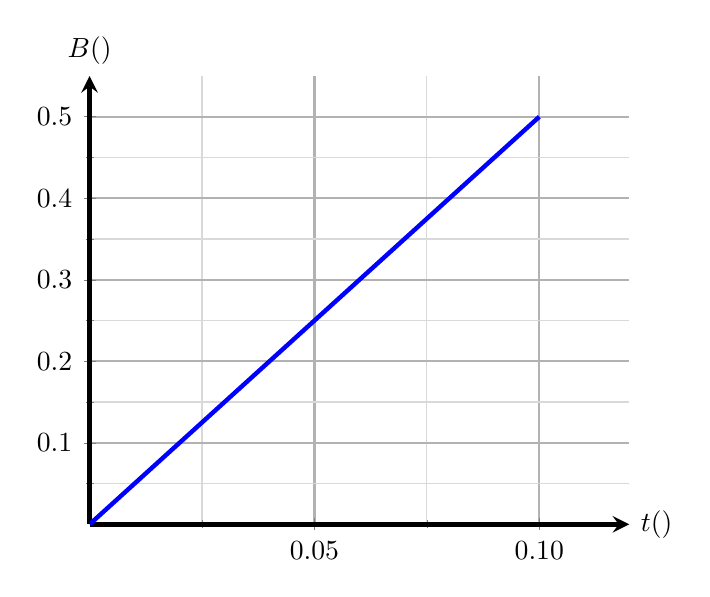
\begin{tikzpicture}  
			\begin{axis}[  ultra thick,
				xmin=0,  
				xmax=0.12,  
				xtick={0,0.05,...,0.10},
				ytick={0,0.1,...,0.5},
				minor x tick num=1,
				minor y tick num=1,
				ymin=0,  
				ymax=0.55, 
				samples=300,
				xticklabel style={/pgf/number format/.cd, fixed,
					fixed zerofill, precision=2},
				axis lines=center, 
				grid style={step=1, line width =0.4pt, color=gray!30!white},
				grid=both, %giới hạn ô lưới
				major grid style={line width=0.8pt,gray!60!white},
				xlabel=$\xsi{t}{\left(\si{\second}\right)}$, 		ylabel=$\xsi{B}{\left(\si{\tesla}\right)}$,
				every axis y label/.style={at=(current axis.above origin),anchor=south},  
				every axis x label/.style={at=(current axis.right of origin),anchor=west},]
				\addplot [ultra thick, blue, smooth, domain=0:0.1] {5*x};  
			\end{axis}  
		\end{tikzpicture}
		\captionof{figure}{}
		\label{fig:20P-2}
	\end{center}
	
	\choice
	{\True $\SI{2.5}{\volt}$}
	{$\SI{-5}{\volt}$}
	{$\SI{-2.5}{\volt}$}
	{$\SI{5}{\volt}$}
	\loigiai{
		$$
		\begin{aligned}
			&\text { Độ lớn suất điện động cảm ứng sinh ra trong vòng dây là: }\\
			&|e|=\left|\frac{\Delta \Phi}{\Delta t}\right|=\left|\frac{S\Delta B}{\Delta t}\right|=\left|\frac{0,5 \cdot 0,5}{0,1}\right|=\SI{2.5}{\volt}
		\end{aligned}
		$$
	}
\end{ex}
% ===================================================================
\begin{ex}
	Một khung dây dẫn kín hình vuông có cạnh dài $\SI{10}{\centi\meter}$ gồm 500 vòng được đặt trong từ trường đều sao cho vector đơn vị pháp tuyến của mặt phẳng khung dây cùng phương cùng chiều với vector cảm ứng từ. Điện trở suất và tiết diện của dây kim loại có giá trị lần lượt là $\SI{2E-8}{\ohm\cdot\meter}$ và $\SI{0.4}{\milli\meter^2}$. Giá trị cảm ứng từ biến thiên theo thời gian như đồ thị trong hình \ref{fig:20P-3}. Công suất toả nhiệt sinh ra trong khung dây có giá trị bao nhiêu?
	\begin{center}
		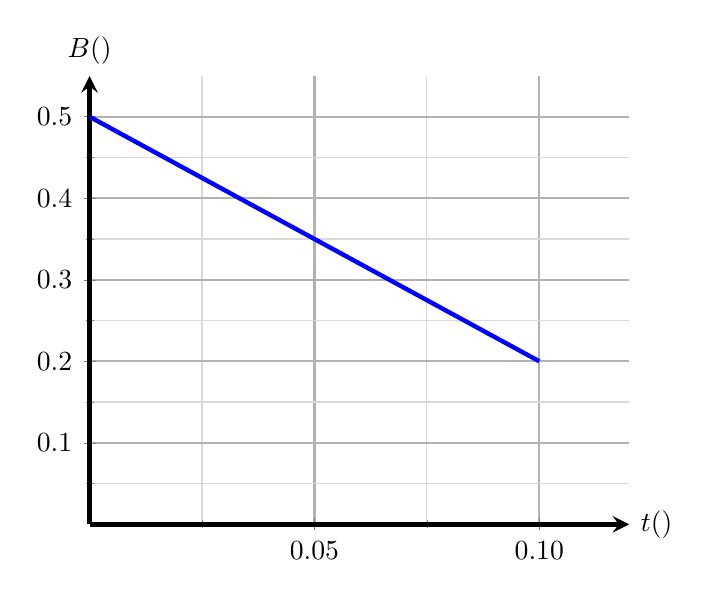
\begin{tikzpicture}  
			\begin{axis}[  ultra thick,
				xmin=0,  
				xmax=0.12,  
				xtick={0,0.05,...,0.10},
				ytick={0,0.1,...,0.5},
				minor x tick num=1,
				minor y tick num=1,
				ymin=0,  
				ymax=0.55, 
				samples=300,
				xticklabel style={/pgf/number format/.cd, fixed,
					fixed zerofill, precision=2},
				axis lines=center, 
				grid style={step=1, line width =0.4pt, color=gray!30!white},
				grid=both, %giới hạn ô lưới
				major grid style={line width=0.8pt,gray!60!white},
				xlabel=$\xsi{t}{\left(\si{\second}\right)}$, 		ylabel=$\xsi{B}{\left(\si{\tesla}\right)}$,
				every axis y label/.style={at=(current axis.above origin),anchor=south},  
				every axis x label/.style={at=(current axis.right of origin),anchor=west},]
				\addplot [ultra thick, blue, smooth, domain=0:0.1] {0.5-3*x};  
			\end{axis}  
		\end{tikzpicture}
		\captionof{figure}{}
		\label{fig:20P-3}
	\end{center}
	\choice
	{$\SI{225}{\milli\watt}$}
	{\True $\SI{22.5}{\watt}$}
	{$\SI{0.09}{\milli\watt}$}
	{$\SI{9}{\watt}$}
	\loigiai{
		Độ lớn suất điện động cảm ứng sinh ra trong khung dây là:
		$$
		|e|=N\left|\frac{\Delta \Phi}{\Delta t}\right|=N S\left|\frac{\Delta B}{\Delta t}\right|=500\cdot0,1^2 \cdot\left|\frac{0,2-0,5}{0,1}\right|=\SI{15}{\volt}
		$$
		Gọi tiết diện của dây kim loại là $S^{\prime}$. Điện trở của dây kim loại trong khung dây là:
		$$
		R=\rho \frac{\ell}{S^{\prime}}=2 \cdot 10^{-8} \cdot \frac{500 \cdot 0,1 \cdot 4}{0,4 \cdot 10^{-6}}=\SI{10}{\ohm}.
		$$
		Công suất toả nhiệt trong khung dây: $\calP=\frac{|e|^2}{R}=\frac{15^2}{10}=\SI{22.5}{\watt}$.
	}
\end{ex}

% ===================================================================
\begin{ex}
	Một khung dây dẫn kín có 500 vòng được đặt trong từ trường đều có độ lớn cảm ứng từ là $\SI{0.4}{\tesla}$. Diện tích mỗi vòng dây là $\SI{50}{\centi\meter^2}$. Cho khung dây quay đều quanh trục vuông góc với vector cảm ứng từ với tốc độ góc là $\xsi{\dfrac{\pi}{3}}{\radian/\second}$. Nối khung dây với tụ điện thì tụ điện tích được một lượng điện tích là $\SI{3}{\micro\coulomb}$. Giả sử điện trở của khung dây là không đáng kể và ban đầu vector cảm ứng từ cùng phương, cùng chiều với vector đơn vị pháp tuyến của mặt phẳng khung dây. Điện dung của tụ điện có giá trị là 
	\choice
	{$\SI{3}{\farad}$}
	{$\SI{3}{\micro\farad}$}
	{$\SI{6}{\farad}$}
	{\True $\SI{6}{\micro\farad}$}
	\loigiai{
		Khung dây quay đều quanh trục vuông góc với vector cảm ứng từ với tốc độ góc là $\xsi{\frac{\pi}{3}}{\radian/\second}$, nghĩa là trong $\SI{1}{\second}$ khung dây quay được một góc là $\xsi{\dfrac{\pi}{3}}{\radian}$.\\
		Độ lớn suất điện động cảm ứng trung bình sinh ra trong khung dây có giá trị là:
		$$
		\begin{aligned}
			|e|=N\left|\frac{\Delta \Phi}{\Delta t}\right|&=N\left|\frac{B S[\cos (\alpha+\omega t)-\cos \alpha]}{\Delta t}\right| \\
			& =500\left|\frac{0,4 \cdot 5 \cdot 10^{-3}\left(\cos \frac{\pi}{3}-\cos 0\right)}{1}\right|=\SI{0.5}{\volt}
		\end{aligned}
		$$
		Vì khung dây có điện trở không đáng kể nên $|e|=U$. Từ công thức tính điện tích của tụ điện, suy ra:
		$$
		Q=C U \Rightarrow C=\frac{Q}{U}=\frac{3}{0,5}=\SI{6}{\micro\farad}.
		$$
	}
\end{ex}

% ===================================================================
\begin{ex}
	Trường hợp nào trong hình bên dưới xác định đúng chiều dòng điện cảm ứng trong khung dây dẫn?
	\choice
	{\True \includegraphics[width=0.4\linewidth]{figs/VN12-Y24-PH-SYL-020P-15a}}
	{\includegraphics[width=0.4\linewidth]{figs/VN12-Y24-PH-SYL-020P-15b}}
	{\includegraphics[width=0.4\linewidth]{figs/VN12-Y24-PH-SYL-020P-15c}}
	{\includegraphics[width=0.4\linewidth]{figs/VN12-Y24-PH-SYL-020P-15d}}
	\loigiai{}
\end{ex}

\Closesolutionfile{ans}
\subsubsection{Trắc nghiệm đúng/sai}
\Opensolutionfile{ans}[ans/VN12-Y24-PH-SYL-020P-TF]
\setcounter{ex}{0}
% ===================================================================
\begin{ex}
	Nối hai đầu cuộn dây dẫn kín với điện kế và cho chuyển động rơi tự do qua một nam châm như hình \ref{fig: 20P-10}. Biết cảm ứng từ, đường sức từ của nam châm được mô tả như hình vẽ và khi bắt đầu chuyển động, kim điện kế chỉ vạch số 0.
	\begin{center}
		\includegraphics[width=0.2\linewidth]{figs/VN12-Y24-PH-SYL-020P-10}
		\captionof{figure}{}
		\label{fig: 20P-10}
	\end{center}
	Các nhận định sau đây là đúng hay sai?
	\choiceTF[t]
	{Cuộn dây rơi tự do nên kim điện kế không bị lệch khỏi vạch số 0 khi đi qua đầu trên của nam châm}
	{Thời điểm cuộn dây rơi đến giữa nam châm thì kim điện kế bị lệch xa nhất khỏi vạch số 0}
	{Thời điểm cuộn dây rơi ra khỏi đầu dưới của nam châm thì kim điện kế chỉ vạch số 0}
	{Chiều dòng điện cảm ứng xuất hiện tại thời điểm cuộn dây đi vào nam châm và cuộn dây đi ra khỏi nam châm là như nhau}
	\loigiai{
		
	}
\end{ex}
% ===================================================================
\begin{ex}
	Đặt hai cuộn dây dẫn kín cạnh nhau, như hình \ref{fig: 20P-11}. Một cuộn nối với nguồn điện. Một cuộn nối với điện kế, khi không có dòng điện chạy trong cuộn dây thì kim điện kế chỉ vạch số 0.
	\begin{center}
		\includegraphics[width=0.3\linewidth]{figs/VN12-Y24-PH-SYL-020P-11}
		\captionof{figure}{}
		\label{fig: 20P-11}
	\end{center}
	Các nhận định sau đây là đúng hay sai?
	\choiceTF[t]
	{\True Kim điện kế bị lệch khỏi vạch số 0 khi nguồn điện là nguồn xoay chiều}
	{Kim điện kế bị lệch khỏi vạch số 0 khi nguồn điện là nguồn điện một chiều}
	{Mắc cuộn dây với nguồn điện một chiều và dịch chuyển cuộn dây ra xa thì kim điện kế không bị lệch khỏi vạch số 0}
	{\True Mắc cuộn dây (1) với nguồn một chiều và dùng tay bóp bẹp cuộn dây 2 thì kim điện kế sẽ bị lệch khỏi vạch số 0}
	\loigiai{}
\end{ex}
% ===================================================================
\begin{ex}
	Một cuộn dây đồng gồm nhiều vòng đặt gần một nam châm thẳng.
	\begin{center}
		\includegraphics[width=0.3\linewidth]{figs/VN12-Y24-PH-SYL-020P-24}
	\end{center}
	Cuộn dây được di chuyển theo hướng mũi tên thể hiện trong sơ đồ.
	\choiceTF[t]
	{Dòng điện cảm ứng trong cuộn dây chạy từ B đến A}
	{Nếu đổi cực nam châm thì trong cuộn dây sẽ không có dòng điện cảm ứng}
	{\True Khi di chuyển cuộn dây nhanh lên thì dòng điện trong cuộn dây sẽ tăng lên}
	{Nếu cho cuộn dây và nam châm di chuyển cùng chiều với cùng tốc độ thì dòng điện cảm ứng trong cuộn dây là dòng điện không đổi}
	\loigiai{
		\begin{itemchoice}
			\itemch Sai. Di chuyển cuộn dây lại gần nam châm thì từ thông qua cuộn dây tăng nên dòng điện cảm ứng trong cuộn dây có chiều sao cho từ trường do nó sinh ra ngược chiều từ trường của nam châm. Do $\vec{B}$ của nam châm hướng sang trái nên $\vec{B}_c$ do dòng điện cảm ứng trong cuộn dây sinh ra hướng sang phải $\Rightarrow$ Mặt B của cuộn dây là mặt Bắc và mặt A của cuộn dây là mặt Nam $\rightarrow$ Dòng điện cảm ứng cùng chiều kim đồng hồ nhìn từ mặt A nên chạy từ A đến B.
			\itemch Sai. Khi đổi cực nam châm và cuộn dây di chuyển lại gần nam châm thì từ thông qua cuộn dây vẫn biến thiên và sinh ra dòng điện cảm ứng.
			\itemch Đúng. Khi di chuyển cuộn dây nhanh lên thì tốc độ biến thiên từ thông qua cuộn dây sẽ tăng lên $\rightarrow$ dòng điện trong cuộn dây sẽ tăng lên.
			\itemch Sai. Lúc này không có sự biến thiên từ thông qua cuộn dây nên không có dòng điện cảm ứng.
			
		\end{itemchoice}	
	}
\end{ex}
% ===================================================================
\begin{ex}
	Một cuộn dây được nối với vôn kế, một nam châm được giữ phía trên cuộn dây.
	\begin{center}
		\includegraphics[width=0.3\linewidth]{figs/VN12-Y24-PH-SYL-021-8}
	\end{center}	
	\choiceTF[t]
	{\True Khi thả cho nam châm rơi vào cuộn dây, kim vôn kế bị lệch}
	{Nếu nam châm được thả từ độ cao lớn hơn, số chỉ cực đại trên vôn kế vẫn như khi nam châm được thả từ độ cao thấp hơn}
	{Khi cuộn dây có nhiều vòng dây hơn, số chỉ trên vôn kế sẽ giảm}
	{Nếu cực Nam của nam châm đi vào cuộn dây trước, kim chỉ trên vôn kế vẫn lệch như khi cực Bắc của nam châm rơi vào cuộn dây trước}
	\loigiai{
		\begin{itemchoice}
			\itemch Đúng. Khi nam châm rơi, từ thông qua cuộn dây thay đổi, sinh ra dòng điện cảm ứng. Sự thay đổi này gây ra suất điện động cảm ứng làm kim vôn kế lệch.
			\itemch Sai. Khi nam châm rơi từ độ cao lớn hơn, nó sẽ tăng tốc khi đi qua cuộn dây do đó tốc độ thay đổi từ thông tăng lên làm tăng số chỉ cực đại trên vôn kế.
			\itemch Sai. Cuộn dây có nhiều vòng dây hơn sẽ tạo ra suất điện động cảm ứng lớn hơn khi nam châm di chuyển qua, dẫn đến số chỉ trên vôn kế sẽ tăng.
			\itemch Sai. Số chỉ trên vôn kế sẽ ngược lại.
			
		\end{itemchoice}	
	}
\end{ex}

% ===================================================================
\begin{ex}
	Một khung kim loại hình tròn đường kính $\SI{5}{\centi\meter}$ được đặt trong vùng từ trường đều có các đường sức từ vuông góc với mặt phẳng khung dây. Hai đầu của khung dây được nối với một bóng đèn nhỏ tạo thành mạch kín. Lấy $\pi \approx 3,14$; biết điện trở của khung kim loại và bóng đèn lần lượt là $R_1=\SI{2}{\ohm}$ và $R_2=\SI{1}{\ohm}$. Tại thời điểm ban đầu $(t=\SI{0}{\second})$, người ta bắt đầu thay đổi độ lớn cảm ứng từ theo đồ thị như hình \ref{fig:20P-4}. Trong mỗi phát biểu sau, em hãy chọn đúng hoặc sai.	
	\begin{center}
		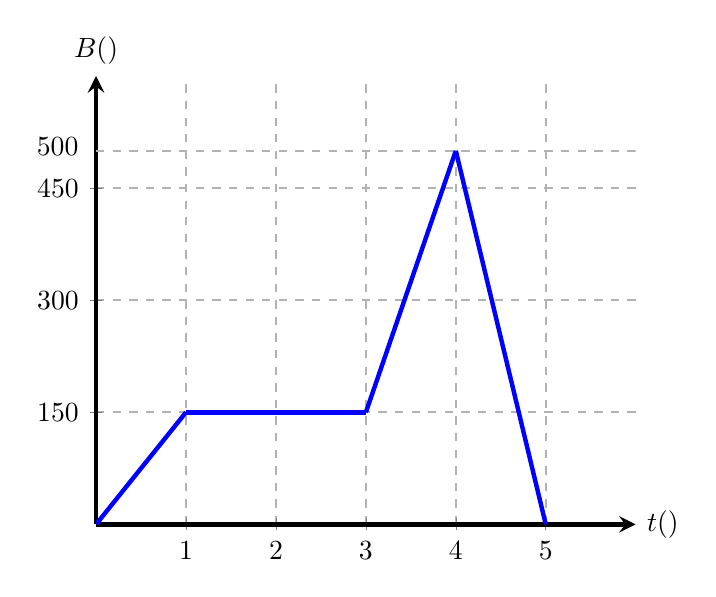
\begin{tikzpicture}  
			\begin{axis}[  ultra thick,
				xmin=0,  
				xmax=6,  
				xtick={0,1,...,5},
				ytick={0,150,...,500},
				minor x tick num=0,
				minor y tick num=0,
				ymin=0,  
				ymax=600, 
				samples=300,
				axis lines=center, 
				grid style={step=1, line width =0.4pt, color=gray!30!white},
				grid=both, %giới hạn ô lưới
				major grid style={line width=0.8pt,gray!60!white, dashed},
				xlabel=$\xsi{t}{\left(\si{\second}\right)}$, 		ylabel=$\xsi{B}{\left(\si{\milli\tesla}\right)}$,
				every axis y label/.style={at=(current axis.above origin),anchor=south},  
				every axis x label/.style={at=(current axis.right of origin),anchor=west},  ]
				\draw[line width =0.8pt, color=gray!60!white, dashed] (axis cs: 0,500)--(axis cs: 6,500);
				\addplot [ultra thick, blue, smooth, domain=0:1] {150*x};  
				\addplot [ultra thick, blue, smooth, domain=1:3] {150}; 
				\addplot [ultra thick, blue, smooth, domain=3:4] {150+350*(x-3)};
				\addplot [ultra thick, blue, smooth, domain=4:5] {500-500*(x-4)}; 
			\end{axis}  
			\node[left] at (-0.1,4.8) {500};
		\end{tikzpicture}
		\captionof{figure}{}
		\label{fig:20P-4}
	\end{center}
	
	\choiceTFt
	{\True Tại thời điểm $t=\SI{0}{\second}$, không có từ thông xuyên qua khung kim loại}
	{\True Tổng thời gian đèn sáng trong quá trình thay đổi nói trên là $\SI{3}{\second}$}
	{Mặc dù dòng điện cảm ứng chạy qua đèn trong khoảng thời gian từ $t=\SI{3}{\second}$ đến $t=\SI{4}{\second}$ và từ $t=\SI{4}{\second}$ đến $t=\SI{5}{\second}$ ngược chiều nhau nhưng cường độ dòng điện có cùng độ lớn}
	{Suất điện động cảm ứng sinh ra trong khoảng thời gian từ $t=\SI{0}{\second}$ đến $t=\SI{1}{\second}$ là $\SI{1.1775E-3}{\volt}$}
	{Độ sáng của đèn trong khoảng thời gian từ $t=\SI{0}{\second}$ đến $t=\SI{1}{\second}$ mạnh hơn trong khoảng thời gian từ $t=\SI{3}{\second}$ đến $t=\SI{4}{\second}$}
	{\True Nhiệt lượng toả ra trên bóng đèn trong một giây cuối cùng của quá trình thay đổi độ lớn cảm ứng từ xấp xỉ $\SI{1.1E-7}{\joule}$}
	\loigiai{
	}
\end{ex}
\Closesolutionfile{ans}
\subsubsection{Tự luận}
\setcounter{ex}{0}
\Opensolutionfile{ans}[ans/VN12-Y24-PH-SYL-020P-TL]
% ======================================================================
\begin{ex}
	Đoạn dây dẫn ở hình \ref{fig:20P-19} là một phần của mạch điện kín. Khi nâng đoạn dây dẫn thẳng đứng lên trên, trong đoạn dây xuất hiện dòng điện cảm ứng. Dòng điện cảm ứng trong đoạn dây dẫn sẽ thay đổi thế nào khi
	\begin{center}
		\includegraphics[width=0.2\linewidth]{figs/VN12-Y24-PH-SYL-020P-19}
		\captionof{figure}{}
		\label{fig:20P-19}
	\end{center}
	\begin{enumerate}[label=\alph*)]
		\item Di chuyển đoạn dây dẫn thẳng đứng xuống dưới?
		\item Giữ đoạn dây dẫn nằm yên?
		\item Di chuyển đoạn dây dẫn song song với đường sức từ?
	\end{enumerate}
	
	\loigiai{
		\begin{enumerate}[label=\alph*)]
			\item Dòng điện đảo chiều.
			\item Không có dòng điện cảm ứng.
			\item Không có dòng điện cảm ứng.
		\end{enumerate}	
	}
\end{ex}
% ======================================================================
\begin{ex}
	Giải thích vì sao thời gian quay của một đĩa nhôm giữa hai cực từ của một nam châm lại nhỏ hơn khi không có nam châm?
	\loigiai{
		Dòng điện xoáy sinh ra trong đĩa tạo ra từ trường cản trở chuyển động.	
	}
\end{ex}

% ======================================================================
\begin{ex}
	Cho một khung kim loại gồm 1000 vòng dây có diện tích $\SI{25}{\centi\meter^2}$ quay quanh trục trong một từ trường đều với độ lớn cảm ứng từ là $\SI{0.01}{\tesla}$ như hình \ref{fig:20P-5}a. Hình \ref{fig:20P-5}b biểu diễn vị trí của khung tại một số thời điểm khác nhau trong quá trình quay so với vector cảm ứng từ. Giá trị góc $\alpha$ hợp bởi vector cảm ứng từ $\vec{B}$ và vector đơn vị pháp tuyến của mặt phẳng khung dây $\vec{n}$ tại một số thời điểm được ghi lại trong bảng bên dưới. Hãy xác định giá trị của từ thông tương ứng với các trường hợp được liệt kê trong hình \ref{fig:20P-4}.
	\begin{center}
		\includegraphics[width=0.9\linewidth]{figs/VN12-Y24-PH-SYL-020P-5}
		\captionof{figure}{}
		\label{fig:20P-5}
	\end{center}
	\begin{center}
		\begin{tabular}{|M{2.5cm}|M{1.25cm}|M{1.25cm}|M{1.25cm}|M{1.25cm}|M{1.25cm}|M{1.25cm}|M{1.25cm}|M{1.25cm}|M{1.25cm}|}
			\hline
			\thead{Thời điểm}&(1)& (2)&(3)&(4)& (5)& (6)& (7)&(8)&(9)\\
			\hline
			$\alpha$&$\SI{0}{\degree}$&$\SI{45}{\degree}$&$\SI{90}{\degree}$&$\SI{135}{\degree}$&$\SI{180}{\degree}$&$\SI{135}{\degree}$&$\SI{90}{\degree}$&$\SI{45}{\degree}$&$\SI{0}{\degree}$\\
			\hline
			$\xsi{\Phi}{\left(\weber\right)}$&&&&&&&&&\\
			\hline
		\end{tabular}
	\end{center}
	\loigiai{
		Áp dụng công thức $\Phi=NBS\cos\alpha$, ta được các giá trị của từ thông trong bảng sau:
		\begin{center}
			\begin{tabular}{|M{2.5cm}|M{1.25cm}|M{1.25cm}|M{1.25cm}|M{1.25cm}|M{1.25cm}|M{1.25cm}|M{1.25cm}|M{1.25cm}|M{1.25cm}|}
				\hline
				\thead{Thời điểm}&(1)& (2)&(3)&(4)& (5)& (6)& (7)&(8)&(9)\\
				\hline
				$\alpha$&$\SI{0}{\degree}$&$\SI{45}{\degree}$&$\SI{90}{\degree}$&$\SI{135}{\degree}$&$\SI{180}{\degree}$&$\SI{135}{\degree}$&$\SI{90}{\degree}$&$\SI{45}{\degree}$&$\SI{0}{\degree}$\\
				\hline
				$\xsi{\Phi}{\left(\weber\right)}$&0,025&$\dfrac{\sqrt{2}}{80}$&0&$-\dfrac{\sqrt{2}}{80}$&$-0,025$&$-\dfrac{\sqrt{2}}{80}$&0&$\dfrac{\sqrt{2}}{80}$&0,025\\
				\hline
			\end{tabular}
		\end{center}
	}
\end{ex}
% ======================================================================
\begin{ex}
	Xét một sóng điện từ đang lan truyền trong không gian với thành phần điện trường tại một điểm A biến thiên điều hoà theo phương trình $E=1,5 \sin (120 t+\pi)\ \left(\si{\volt/\meter}\right)$.
	\begin{enumerate}[label=\alph*)]
		\item Hãy xác định tần số góc và pha ban đầu trong sự biến thiên của thành phần từ trường tại điểm A.
		\item Tại thời điểm $t$, cường độ điện trường tại A có giá trị $\SI{1.5}{\volt/\meter}$. Sau khoảng thời gian bằng một phần tư chu kì thì cảm ứng từ tại điểm đó có giá trị bằng bao nhiêu?	
	\end{enumerate}
	\loigiai{
		\begin{enumerate}[label=\alph*)]
			\item Vì cả hai thành phần điện trường và từ trường trong sóng điện từ biến thiên cùng tần số, cùng pha với nhau nên tần số góc và pha ban đầu cần tìm lần lượt là $\omega=\SI{120}{\radian/\second}$ và $\varphi=\xsi{\pi}{\radian}$.
			\item Ta thấy tại thời điểm $t$ cuờng độ điện trường đang đạt giá trị cực đại, suy ra thành phần từ trường cũng đạt giá trị cực đại. Do đó, sau một phần tư chu kì truyền sóng thì giá trị của cảm ứng từ tại điểm đó sẽ bằng không.
		\end{enumerate}
	}
\end{ex}
% ======================================================================
\begin{ex}
	Cho một thanh kim loại ab đang được kéo đều trên đường ray dẫn điện. Cả hệ thống đường ray và thanh ab đang được đặt trong vùng từ trường đều có hướng vuông góc với mặt phẳng khung và có chiều như hình \ref{fig:20P-6}. Trong quá trình thanh di chuyển, từ trường sinh ra bởi dòng điện cảm ứng có chiều hướng như thế nào? Vì sao?
	\begin{center}
		\includegraphics[width=0.4\linewidth]{figs/VN12-Y24-PH-SYL-020P-6}
		\captionof{figure}{}
		\label{fig:20P-6}
	\end{center}
	\loigiai{
		Khi thanh kim loại ab chuyển động sang phải, diện tích giới hạn bởi đường ray và thanh kim loại tăng lên làm cho từ thông tăng dần. Theo định luật Lenz về hiện tượng cảm ứng điện từ, dòng điện cảm ứng sinh ra có chiều chống lại nguyên nhân sinh ra nó, tức là từ trường sinh ra bởi dòng điện này phải có tác dụng làm giảm sự tăng lên của từ thông. Chính vì vậy các đường sức từ của từ trường do dòng điện cảm ứng sinh ra hướng ngược lại với các đường sức từ ban đầu.
	}
\end{ex}
% ======================================================================
\begin{ex}
	Một dây dẫn bằng sắt được uốn thành vòng tròn và đang được đặt trong vùng từ trường đều với các đường sức từ hướng vuông góc với mặt phẳng vòng dây như hình \ref{fig:20P-8}. Hãy mô tả chiều của dòng điện cảm ứng sinh ra trong các trường hợp dưới đây:
	\begin{center}
		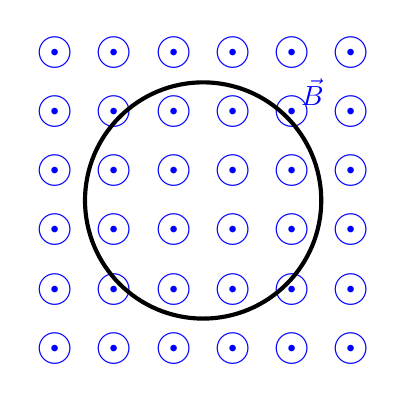
\begin{tikzpicture}
			\foreach \x in {0,0.75,...,3.75}{
				\foreach \y in {0,0.75,...,3.75}{
					\node[blue] at (\x, \y) {\LARGE$\odot$};
				}
			}
			\node[blue, right] at(3,3.25) {$\vec{B}$};
			\draw[line width=1.5pt] (1.875,1.875) circle (1.5);
		\end{tikzpicture}
		\captionof{figure}{}
		\label{fig:20P-8}
	\end{center}
	\begin{enumerate}[label=\alph*)]
		\item Trường hợp 1: Độ lớn cảm ứng từ được điều chỉnh giảm dần theo thời gian.
		\item Trường hợp 2: Độ lớn cảm ứng từ được điều chỉnh tăng dần theo thời gian.
		\item Trường hợp 3: Từ vị trí ban đầu, tịnh tiến vòng kim loại sang trái (vòng kim loại vẫn nằm trong vùng từ trường).
	\end{enumerate}
	\loigiai{
		\begin{enumerate}[label=\alph*)]
			\item Sự giảm dần của độ lớn cảm ứng từ dẫn đến số đường sức từ xuyên qua mặt phẳng vòng dây giảm dần, do đó từ thông qua vòng dây giảm và trong vòng dây xuất hiện dòng điện cảm ứng. Từ trường sinh ra bởi dòng điện cảm ứng sẽ hướng vuông góc với mặt phẳng vòng kim loại và hướng ra khỏi mặt giấy (theo định luật Lenz về hiện tượng cảm ứng điện từ). Dựa vào quy tắc nắm tay phải, dòng điện cảm ứng sẽ hướng ngược chiều kim đồng hồ.	
			\item Lập luận tương tự như câu a, ta thấy lúc này dòng điện cảm ứng hướng cùng chiều kim đồng hồ.
			\item Vì từ thông xuyên qua vòng dây không đổi theo thời gian nên không có dòng điện cảm ứng xuất hiện trong vòng kim loại.
		\end{enumerate}
	}
\end{ex}
% ======================================================================
\begin{ex}
	Một hình vuông cạnh $\SI{5}{\centi\meter}$ đặt trong từ trường đều có cảm ứng từ $B=\SI{8E-4}{\tesla}$. Từ thông qua hình vuông đó bằng $\SI{E-6}{\weber}$. Tính góc hợp bởi vector cảm ứng từ với mặt phẳng của hình vuông đó.
	\loigiai{
		Diện tích khung dây: $S=\SI{25E-4}{\meter^2}$.\\
		Áp dụng công thức tính từ thông: $\Phi=BS \cos \alpha \Rightarrow \cos \alpha=\frac{1}{2} \Rightarrow \alpha= \pm \xsi{\frac{\pi}{3}}{\radian}$. \\
		Trong đó $\alpha$ là góc tạo bởi vector pháp tuyến của mặt phẳng hình vuông và vector cảm ứng từ, nên góc tạo bởi vector cảm ứng từ với mặt phẳng hình vuông là: $\beta=\dfrac{\pi}{2}-\alpha=\xsi{\dfrac{\pi}{6}}{\radian}$ hoặc $\xsi{\dfrac{5 \pi}{6}}{\radian}$.\\
		Do góc hợp bởi vector cảm ứng từ với mặt phẳng của hình vuông là góc nhọn, nên chọn $\beta=\xsi{\dfrac{\pi}{6}}{\radian}$.
	}
\end{ex}
% ======================================================================
\begin{ex}
	Một khung dây dẫn gồm 200 vòng có diện tích $\SI{8.5}{\centi\meter^2}$ và mặt phẳng khung dây vuông góc với cảm ứng từ có độ lớn thay đổi từ $\SI{0.03}{\tesla}$ đến $\SI{0.12}{\tesla}$ trong $\SI{15}{\milli\second}$. Tính độ lớn suất điện động cảm ứng trong khung dây.
	\loigiai{
		Độ lớn suất điện động cảm ứng:
		$$\left|e\right|=\left|\dfrac{NS\Delta B}{\Delta t}\right|=\SI{1.02}{\volt}.$$	
	}
\end{ex}
% ======================================================================
\begin{ex}
	Một vòng dây dẫn phẳng hình tròn có diện tích $S=\SI{30}{\centi\meter^2}$ ở trong một từ trường dều có $B=\SI{0.2}{\tesla}$. Trong $\SI{0.5}{\second}$ vòng dây quay đều được một góc $\SI{60}{\degree}$. Tìm:
	\begin{center}
		\includegraphics[width=0.3\linewidth]{figs/VN12-Y24-PH-SYL-020P-21}
	\end{center}
	\begin{enumerate}[label=\alph*)]
		\item độ lớn suất điện động cảm ứng trong vòng dây.
		\item chiều của dòng điện cảm ứng trong vòng dây.
	\end{enumerate}
	\loigiai{
		\begin{enumerate}[label=\alph*)]
			\item $\SI{6E-4}{\volt}$
			\item dòng điện có hướng ngược chiều kim đồng hồ (nhìn từ trên xuống vòng dây).
		\end{enumerate}	
	}
\end{ex}
% ======================================================================
\begin{ex}
	Một khung dây kín có 100 vòng, mỗi vòng có diện tích là $\SI{80}{\deci\meter^2}$. Vòng dây được đặt trong từ trường đều sao cho vector cảm ứng từ hợp với vector đơn vị pháp tuyến của mặt phẳng khung dây một góc $\alpha$. Độ lớn cảm ứng từ biến thiên theo thời gian như đồ thị trong hình \ref{fig:20P-7}. Độ lớn suất điện động cảm ứng trong vòng dây có giá trị là $\SI{40}{\volt}$. Góc $\alpha$ có giá trị là bao nhiêu?
	\begin{center}
		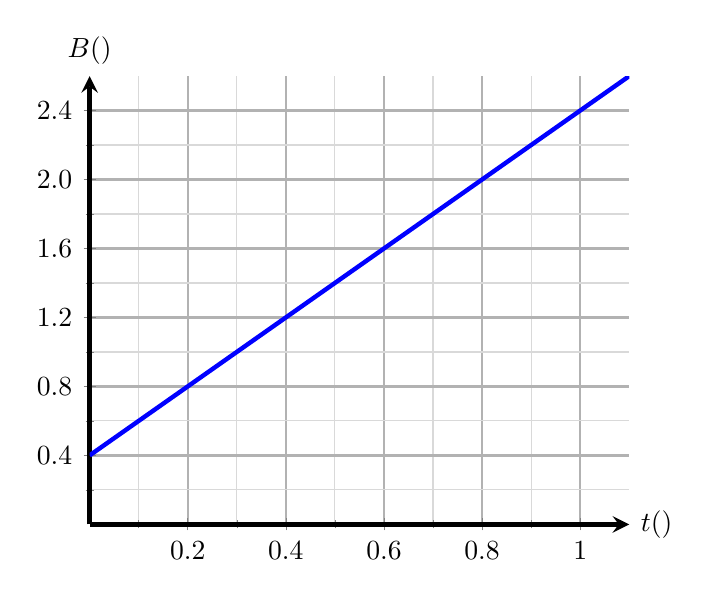
\begin{tikzpicture}  
			\begin{axis}[  ultra thick,
				xmin=0,  
				xmax=1.1,  
				xtick={0,0.2,...,1},
				ytick={0,0.4,...,2.4},
				minor x tick num=1,
				minor y tick num=1,
				ymin=0,  
				ymax=2.6, 
				samples=300,
				yticklabel style={/pgf/number format/.cd, fixed,
					fixed zerofill, precision=1},
				axis lines=center, 
				grid style={step=1, line width =0.4pt, color=gray!30!white},
				grid=both, %giới hạn ô lưới
				major grid style={line width=0.8pt,gray!60!white},
				xlabel=$\xsi{t}{\left(\si{\second}\right)}$, 		ylabel=$\xsi{B}{\left(\si{\tesla}\right)}$,
				every axis y label/.style={at=(current axis.above origin),anchor=south},  
				every axis x label/.style={at=(current axis.right of origin),anchor=west},  ]
				\addplot [ultra thick, blue, smooth, domain=0:6] {0.4+2*x}; 
			\end{axis}  
		\end{tikzpicture}
		\captionof{figure}{}
		\label{fig:20P-7}
	\end{center}
	
	\loigiai{
		Từ biểu thức tính độ lớn suất điện động cảm ứng, ta suy ra giá trị của góc hợp bởi vector cảm ứng từ và vector đơn vị pháp tuyến của mặt phẳng khung dây như sau:
		$$
		\begin{aligned}
			& \left|e\right|=N\left|\frac{\Delta \Phi}{\Delta t}\right|=N \frac{|\Delta B| S \cos \alpha}{\Delta t} \\
			\Rightarrow & \cos \alpha=\frac{|e| \Delta t}{N|\Delta B| S}=\frac{40\cdot1}{100\cdot2 \cdot 0,8}=0,25 \Rightarrow \alpha \approx \SI{75.5}{\degree}
		\end{aligned}
		$$
	}
\end{ex}
% ======================================================================
\begin{ex}
	Một nhóm học sinh dùng ống dây nối với điện kế nhạy có điểm 0 ở giữa để làm thí nghiệm về hiện tượng cảm ứng diện từ. Họ di chuyển một thanh nam châm lại gần một đầu ống dây như hình \ref{fig: 20P-20}. Kim của điện kế lệch sang trái.
	\begin{center}
		\includegraphics[width=0.3\linewidth]{figs/VN12-Y24-PH-SYL-020P-20}
		\captionof{figure}{}
		\label{fig: 20P-20}
	\end{center}
	\begin{enumerate}[label=\alph*)]
		\item Giải thích tại sao kim của điện kế di chuyển.
		\item Hãy đề xuất cách làm cho kim điện kế lệch sang phải.
		\item Nêu cách làm thế nào để có được số chỉ lớn hơn trên điện kế.
		\item Cho biết số chỉ của điện kế sẽ thế nào nếu giữ nam châm đứng yên trong ống dây.
	\end{enumerate}
	\loigiai{
		\begin{enumerate}[label=\alph*)]
			\item Ống dây và từ trường đang chuyển động tương đối với nhau, do đó xuất hiện một suất điện động cảm ứng trong ống dây.
			\item Di chuyển nam châm ra khỏi ống dây hoặc di chuyển ống dây ra khỏi nam châm hoặc đưa cực nam của nam châm vào cùng một đầu của ống dây hoặc đưa cực bắc của nam châm vào đầu kia của ống dây.
			\item Di chuyển nam châm nhanh hơn hoặc sử dụng nam châm mạnh hơn hoặc tăng số vòng trên một đơn vị chiều dài của ống dây.
			\item Kim chỉ số 0.
		\end{enumerate}	
	}
\end{ex}
% ======================================================================
\begin{ex}
	Một cuộn dây dẫn kín, dẹt hình tròn, gồm $\mathrm{N}=100$ vòng, mỗi vòng có bán kính $r=\SI{10}{\centi\meter}$, mỗi mét chiều dài của dây dẫn có điện trở $R_0=\SI{0.5}{\ohm}$. Cuộn dây đặt trong một từ trường đều có vector cảm ứng từ $\vec{B}$ vuông góc với mặt phẳng các vòng dây và có độ lớn $B=\SI{E-2}{\tesla}$ giảm đều đến 0 trong thời gian $\Delta t=\SI{E-2}{\second}$. Tính cường độ dòng điện cảm ứng xuất hiện trong cuộn dây.
	\loigiai{
		Từ thông qua một vòng dây của cuộn dây là: $\Phi=B S \cos \alpha$, trong đó $\alpha=0$ và $S=\pi r^2$. Xét trong khoảng thời gian từ $t_0=0$ đến thời điểm $t$, từ thông qua 1 vòng dây thay đổi từ $\Phi_0$ đến $\Phi_1$ ứng với cảm ứng từ là $B_0=\SI{E-2}{\tesla}$ và $B_t=0$.\\
		Theo định luật Faraday ta có suất điện động cảm ứng qua $N$ vòng dây của cuộn dây là:
		$$
		e=-N \frac{\Delta\Phi}{\Delta t}=-NS \frac{\Delta B}{\Delta t}
		$$\\
		Cường độ dòng điện cảm ứng xuất hiện trong cuộn dây là: $i=\dfrac{e}{R}$\\
		Trong đó, $R=LR_0=N2 \pi rR_0$ là điện trở của khung dây.\\
		Do đó, $i=-N \pi r^2 \dfrac{\dfrac{\Delta B}{\Delta t}}{N 2 \pi rR_0}=-\dfrac{r}{2R_0} \cdot \dfrac{\Delta B}{\Delta t}=-\dfrac{0,1}{2 \cdot 0,5} \cdot \dfrac{0-10^{-2}}{10^{-2}}=\SI{0.1}{\ampere}$.
		
	}
\end{ex}
% ======================================================================
\begin{ex}
	Một khung dây dẫn hình vuông, cạnh $a=\SI{10}{\centi\meter}$, đặt cố định trong từ trường đều có vector cảm ứng từ $\vec{B}$ vuông góc với mặt phẳng khung. Trong khoảng thời gian $\Delta t=\SI{0.05}{\second}$, cho độ lớn của $B$ tăng đều từ 0 đến $\SI{0.5}{\tesla}$. Xác định độ lớn của suất điện động cảm ứng xuất hiện trong khung.
	\loigiai{
		Ta có $\alpha=0$ và $N=1$,\\
		nên $\left|e\right|=\left|-N\dfrac{\Delta \Phi}{\Delta t}\right|=\left|-S\dfrac{\Delta B}{\Delta t}\right|=\left|-0,1^2\cdot\dfrac{0,5}{0,05}\right|=\SI{0.1}{\volt}=\SI{100}{\milli\volt}.$
	}
\end{ex}
% ======================================================================
\begin{ex}
	Để giám sát quá trình hô hấp của bệnh nhân, các nhân viên y tế sử dụng một đai mỏng gồm 250 vòng dây kim loại quấn liên tiếp nhau được buộc xung quanh ngực của bệnh nhân như hình \ref{fig:20P-9}. Khi bệnh nhân hít vào, diện tích của các vòng dây tăng lên một lượng $\SI{45}{\centi\meter^2}$. Biết từ trường Trái Đất tại vị trí đang xét được xem gần đúng là đều và có độ lớn cảm ứng từ xấp xỉ $\SI{56}{\micro\tesla}$, các đường sức từ hợp với mặt phẳng cuộn dây một góc $\SI{32}{\degree}$. Giả sử thời gian để một bệnh nhân hít vào là $\SI{1.5}{\second}$, hãy xác định độ lớn suất điện động cảm ứng trung bình sinh ra bởi cuộn dây trong quá trình nói trên.
	\begin{center}
		\includegraphics[width=0.4\linewidth]{figs/VN12-Y24-PH-SYL-020P-9}
		\captionof{figure}{}
		\label{fig:20P-9}
	\end{center}
	
	\loigiai{
		Độ lớn suất điện động cảm ứng trung bình sinh ra trong quá trình hít vào là:
		$$
		\left|e\right|=N\left|\frac{\Delta \Phi}{\Delta t}\right|=N\left|\frac{B \Delta S \cos \alpha}{\Delta t}\right|=\left|\frac{250 \cdot 56 \cdot 10^{-6} \cdot 45 \cdot 10^{-4} \cdot \cos \left(\SI{90}{\degree}-\SI{32}{\degree}\right)}{1,5}\right| \approx \SI{2.2E-5}{\volt}.
		$$
	}
\end{ex}

% ======================================================================
\begin{ex}
	Một khung dây cứng, phẳng diện tích $\SI{25}{\centi\meter^2}$, gồm 10 vòng dây. Khung dây được đặt trong từ trường đều. Khung dây nằm trong mặt phẳng như hình \ref{fig: 20P-16}. Cảm ứng từ biến thiên theo thời gian như đồ thị.
	\begin{center}
		\includegraphics[width=0.4\linewidth]{figs/VN12-Y24-PH-SYL-020P-16}
		\captionof{figure}{}
		\label{fig: 20P-16}
	\end{center}
	\begin{enumerate}[label=\alph*)]
		\item Tính độ biến thiên của từ thông qua khung dây kể từ lúc $t=0$ đến $t=\SI{0.4}{\second}$.
		\item Xác định suất điện động cảm ứng trong khung.
		\item Tìm chiều của dòng điện cảm ứng trong khung.
	\end{enumerate}
	\loigiai{
		\begin{enumerate}[label=\alph*)]
			\item Tại thời điếm $t_0=0$ thì $B_0=\SI{2.4E-3}{\tesla}$; thời điểm $t=\SI{0.4}{\second}$ thì $B_t=\SI{0}{\tesla}$ và góc $\alpha=0$.\\
			Do đó, ta có $\Delta \Phi=\Phi_1-\Phi_0=NS\cdot \Delta B=10 \cdot 25 \cdot 10^{-4} \cdot\left(-2,4 \cdot 10^{-3}\right)=\SI{-6E-5}{\weber}$.
			\item Theo định luật Faraday ta có: 
			$$e=-\frac{\Delta \Phi}{\Delta t}=\frac{6 \cdot 10^{-5}}{0,4}=\SI{1.5E-4}{\volt}=\SI{0.15}{\milli\volt}.$$
			\item Cảm ứng từ $B$ giảm nên theo định luật Lenz cảm ứng từ do dòng điện cảm ứng sinh ra sẽ cùng chiều với cảm ứng từ $B$. Theo quy tắc bàn tay phải, tìm được chiều dòng điện cảm ứng theo chiều kim đồng hồ chạy trong cuộn dây.
		\end{enumerate}
	}
\end{ex}
% ======================================================================
\begin{ex}
	Một khung dây kín phẳng hình vuông ABCD có cạnh $a=\SI{10}{\centi\meter}$ gồm $N=250$ vòng. Khung chuyển động thẳng đều tiến lại khoảng không gian có từ trường đều. Trong khi chuyển động, cạnh AB và DC luôn nằm trên hai đường thẳng song song như hình \ref{fig: 20P-17}. 
	\begin{center}
		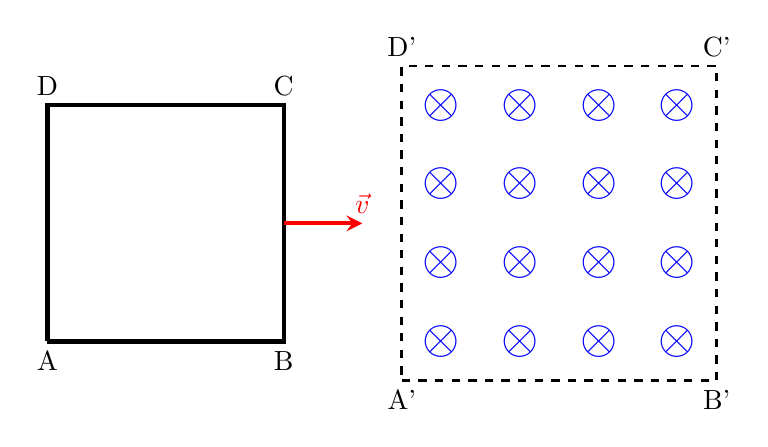
\begin{tikzpicture}
			\coordinate (A) at (-1.5,-1.5);
			\coordinate (B) at (1.5,-1.5);
			\coordinate (C) at (1.5,1.5);
			\coordinate (D) at (-1.5,1.5);
			\coordinate (A') at (3,-2);
			\coordinate (B') at (7,-2);
			\coordinate (C') at (7,2);
			\coordinate (D') at (3,2);
			\foreach \i in {3.5,4.5,5.5,6.5}{
				\foreach \j in {-1.5,-0.5,0.5,1.5}{
					\node[blue] at (\i, \j) {\LARGE $\otimes$};
				}
			};
			\draw[line width=1.5pt] (A)--(B)--(C)--(D)--(A);
			\draw[line width=1pt, dashed] (A')--(B')--(C')--(D')--(A');
			\draw[-stealth, line width=1.5pt, red] (1.5,0)--(2.5,0);
			\node[below] at(A) {A};
			\node[below] at(B) {B};
			\node[above] at(C) {C};
			\node[above] at(D) {D};
			\node[below] at(A') {A'};
			\node[below] at(B') {B'};
			\node[above] at(C') {C'};
			\node[above] at(D') {D'};
			\node[above, red] at (2.5,0) {$\vec{v}$};
		\end{tikzpicture}
		\captionof{figure}{}
		\label{fig: 20P-17}
	\end{center}
	Tính cường độ dòng điện cảm ứng chạy trong khung trong khoảng thời gian từ khi cạnh CB của khung bắt đầu gặp từ trường đến khi khung vừa vặn nằm hẳn trong từ trường. Chỉ rõ chiều dòng điện trong khung. Cho biết điện trở của khung là $\SI{3}{\ohm}$. Tốc độ của khung $v=\SI{1.5}{\meter/\second}$ và cảm ứng từ của từ trường $B=\SI{0.005}{\tesla}$.
	\loigiai{
		Tại thời điểm $t_0=0$ khi khung dây có cạnh BC bắt đầu vào vùng từ trường đếu thì diện tích khung dây nằm trong từ trường $S_0=0$ và thời điểm t thì diện tích khung dây vào trong từ trường là $S_t=BC\cdot vt= avt$ và góc $\alpha=0 \Rightarrow$ từ thông qua 1 vòng của khung dây là $\Phi_t=BS_t=Bav\cdot\Delta t$\\
		Theo định luật Faraday ta có:
		$$
		e=-N \dfrac{\Delta \Phi}{\Delta t}=N \dfrac{Bav \cdot \Delta t}{\Delta t}=NBav=250\cdot 0,005 \cdot 0,1 \cdot 1,5=\SI{0.1875}{\volt}.
		$$
		
		Lại có $$i=\dfrac{e}{R}=\dfrac{NBav}{R}=\dfrac{0,1875}{3}=\SI{0.0625}{\ampere}=\SI{62.5}{\milli\ampere}.$$
		Khi khung dây đi vào vùng từ trường, từ thông qua khung dây tăng, nên cảm ứng từ do dòng điện cảm ứng sinh ra ngược chiều với cảm ứng từ của vùng từ trường, do đó, chiều dòng điện qua khung theo chiều ngược chiều kim đồng hồ hay có chiều từ A đến B .
	}
\end{ex}
% ======================================================================
\begin{ex}
	Một khung dây hình chữ nhật có các cạnh lần lượt là: $a=\SI{10}{\centi\meter}$; $b=\SI{20}{\centi\meter}$ gồm 50 vòng dây quay đều trong một từ trường đều có cảm ứng từ $B=\SI{0.5}{\tesla}$. Trục quay của khung nằm vuông góc với đường sức từ. Lúc đầu, mặt phẳng khung vuông góc với vector cảm ứng từ. Khung quay với tốc độ góc $\omega=\xsi{100\pi}{\radian/\second}$. Tính suất điện động cảm ứng trung bình trong khung dây trong thời gian nó quay được $\SI{15}{\degree}$ kể từ vị trí ban đầu.
	\loigiai{
		Tại thời điểm $t_0=0: \alpha=0$; tại thời điểm $t: \alpha=\omega t=\xsi{\dfrac{\pi}{12}}{\radian}$ nên $t=\xsi{\dfrac{1}{12} \cdot 10^{-2}}{\second}\Rightarrow$ từ thông qua mỗi vòng dây là: $\Phi=BS \cos \alpha$.\\
		Theo định luật Faraday ta có:
		$$
		e=-N \dfrac{\Delta \Phi}{\Delta t}=-NBS \dfrac{\cos \dfrac{\pi}{12}-\cos 0}{\Delta t}=-50\cdot0,5 \cdot 0,1 \cdot 0,2 \dfrac{\cos \dfrac{\pi}{12}-\cos 0}{\dfrac{1}{12} \cdot 10^{-2}}=\SI{20.44}{\volt}.
		$$
	}
\end{ex}
\Closesolutionfile{ans}